\documentclass[12pt]{article}
% Some custom commands to make typing easier. Feel free to add to it


% quick homomorphism
\newcommand{\homo}[1]{\varphi (#1)}
% quick inverse
\newcommand{\inv}[1]{#1^{-1}}
% quick generating set
\newcommand{\genset}[1]{\langle #1 \rangle}
% split problem into multiple parts
\newcommand{\spl}{\rule{\textwidth}{0.4pt}}
% quick normal subgroup
\newcommand{\nsub}{\trianglelefteq}
% quick Z/nZ
\newcommand{\znz}[1]{\mathbb{Z\text{/#1}Z}}

% quick projective surface
\newcommand{\proj}[1]{\mathbb P^{#1}(\mathbb C)}
% quick elliptic curve
\newcommand{\ellip}{E(\mathbb{C})}
% quick ramification
\newcommand{\ram}[1]{e_{#1}}

% quick compactified complex plane
\newcommand{\Chat}{\widehat{\C}}

% todo list
\usepackage[color=yellow]{todonotes}
\newcommand{\tbd}[1]{\todo[inline]{#1}
\addcontentsline{toc}{subsubsection}{TODO}}

% scaling tikz
\usepackage{adjustbox}

% format bullets
% \usepackage[shortlabels]{enumitem}

% Document inherent packages to be loaded
\usepackage{amsmath, amsfonts, amssymb, amsthm, graphicx, url, xcolor, enumerate, tcolorbox}

%geometry helps manage margins, among other things.
\usepackage[rmargin=2in,lmargin=1in,tmargin=1in,bmargin=1in]{geometry}
\newcommand{\sidenote}[1]{\marginpar{\footnotesize \begin{itemize}
    \item[$\leftarrow$]\raggedright #1
\end{itemize}}}

\setlength{\headheight}{16pt}
\setlength{\marginparwidth}{1.5in}
\makeatletter      % make title smaller   
\def\@maketitle{   % custom maketitle 
\begin{center}
    {\Large \@title} \\[0.1in] \@author \\ {\small \@date}
\end{center}  
}
\setcounter{secnumdepth}{0}

\usepackage[colorlinks = true,
            linkcolor = teal,
            urlcolor  = teal,
            citecolor = teal,
            anchorcolor = teal]{hyperref}

\usepackage[all,2cell,ps]{xy}
\usepackage{tikz, tikz-cd}
\usepackage{faktor}
\allowdisplaybreaks
\graphicspath{{Images/}}

\theoremstyle{definition}  % to get rid of the italics
\newtheorem{theorem}{\bt{Theorem}}%[section]
\newtheorem{proposition}[theorem]{\bt{Proposition}}
\newtheorem{corollary}[theorem]{\gt{Corollary}}
\newtheorem{lemma}[theorem]{\bt{Lemma}}
\newtheorem{conjecture}[theorem]{Conjecture}

\newtheorem{defn}{\rt{Definition}}

\newtheorem{eg}{\textcolor{violet}{Example}}
\newtheorem{noneg}[eg]{\textcolor{violet}{Non-example}}

\newtheorem*{rmk}{Remark}


%Import the natbib package and sets a bibliography  and citation styles
\usepackage{natbib}

% Create headers
\usepackage{fancyhdr}
\usepackage{xcolor}
\renewcommand{\headrulewidth}{0pt}
\fancypagestyle{updated}{%
    \fancyhead{MATH135 Notes \hfill\hfill Xuehuai He}
    \fancyfoot{\hyperlink{toc}{Back to TOC}\hfill\thepage \hfill \textcolor{lightgray}{\today}}
}

% \newcommand{\Belyi}{Bely\u{\i}~}
% \newcommand{\thm}[3]{\vskip 0.2in \begin{center} \fbox{\begin{minipage}{0.8\linewidth} \begin{theorem}[#1] \label{#2} #3 \end{theorem} \end{minipage}} \end{center} \vskip 0.2in}
% \newcommand{\prop}[3]{\vskip 0.2in \begin{center} \fbox{\begin{minipage}{0.8\linewidth} \begin{proposition}[#1] \label{#2} #3 \end{proposition} \end{minipage}} \end{center} \vskip 0.2in}
% \newcommand{\cor}[3]{\vskip 0.2in \begin{center} \fbox{\begin{minipage}{0.8\linewidth} \begin{corollary}[#1] \label{#2} #3 \end{corollary} \end{minipage}} \end{center} \vskip 0.2in}
% \newcommand{\conj}[3]{\vskip 0.2in \begin{center} \fbox{\begin{minipage}{0.8\linewidth} \begin{conjecture}[#1] \label{#2} #3 \end{conjecture} \end{minipage}} \end{center} \vskip 0.2in}

\DeclareMathOperator{\Aut}{Aut}
\DeclareMathOperator{\Gal}{Gal}
\DeclareMathOperator{\Mon}{Mon}
\DeclareMathOperator{\lcm}{lcm}
\DeclareMathOperator{\Res}{Res}


\newcommand{\rt}[1]{\textcolor{magenta}{#1}}
\newcommand{\gt}[1]{\textcolor{olive}{#1}}
\newcommand{\bt}[1]{\textcolor{cyan}{#1}}

\newcommand{\N}{\mathbb{N}}
\newcommand{\Z}{\mathbb{Z}}
\newcommand{\C}{\mathbb{C}}
\newcommand{\R}{\mathbb{R}}
\newcommand{\Q}{\mathbb{Q}}
\newcommand{\F}{\mathbb{F}}
\newcommand{\D}{\mathbb{D}}
\newcommand{\reg}{\Omega}

\newcommand{\re}{\operatorname{Re}}
\newcommand{\im}{\operatorname{Im}}
\newcommand{\floor}[1]{\lfloor #1\rfloor}

\newcommand{\ifnif}{\textit{if and only if }}

\newcommand{\addlink}[1]{\addcontentsline{toc}{subsubsection}{#1}}

\newcommand{\circled}[1]{\begin{tikzpicture}[baseline=(word.base)]
\node[draw, rounded corners, text height=8pt, text depth=2pt, inner sep=2pt, outer sep=0pt, use as bounding box] (word) {#1};
\end{tikzpicture}
}

\newcommand{\ontangent}[1]{

    \spl

\textcolor{darkgray}{\textit{(Scratch work begins)}}
{#1}
\textcolor{darkgray}{\textit{(Scratch ends here)}}

\spl

}

\newcommand{\drawing}[2]{\begin{figure}[H]
    \centering
    \includegraphics[width=#1]{Images/#2}
\end{figure}}

\usepackage{pgfplots}
\pgfplotsset{compat=1.15}

\usepackage{ulem}
\usepackage{float}
\usepackage{libertinus}

% Make enumeration better
\usepackage{enumitem}
\setlist[itemize]{parsep=0pt,topsep=0pt}
\setlist[enumerate]{parsep=0pt,topsep=0pt}

% \definecolor{pomona}{HTML}{#0057b8}

\parskip = .2in
\parindent = 0in

% clever ref (load last)
\usepackage[capitalise]{cleveref}
\newcommand{\fref}{\cref}
\newcommand{\Fref}{\Cref}
\newcommand{\prettyref}{\cref}
\newcommand{\newrefformat}[2]{}

 %Cleveref definitions
\crefname{lemma}{Lemma}{Lemmas}
\crefname{thm}{Theorem}{Theorems}
\crefname{defn}{Definition}{Definitions}
\crefname{notn}{Notation}{Notations}
\crefname{const}{Construction}{Constructions}
\crefname{prop}{Proposition}{Propositions}
\crefname{rem}{Remark}{Remarks}
\crefname{cor}{Corollary}{Corollaries}
\crefname{equation}{Equation}{Equations}
\crefname{ex}{Example}{Examples}

%=============

\begin{document}
\title{MATH135 Complex Analysis Notes}
\author{Xuehuai He}
\maketitle

\hypertarget{toc}{}
{\parskip=0.05in
\tableofcontents}

\spl

\newpage
\pagestyle{updated}

\section{Regions, differentiability, analyticity}

\subsection{Regions}
\defn A \textbf{region} is a \uline{nonempty, connected, open subset} of $\C$.
\begin{itemize}
    \item A region without ``holes'' is \uline{simply connected}.
\end{itemize}

\noneg This is not a region (not connected): \drawing{80pt}{image.png}

\eg $\C$ is a region.
\eg $\mathbb{D} = \{z\in \C\mid |z|<1\}$, the open unit disk is a region.
\eg $\{z\in \C \mid 1<|z|<2\}$, the annulus region is a region that is not \textit{simply-connected}:\drawing{80pt}{image-1.png}

\subsection{Complex derivatives and analyticity}

\defn Let $\reg$ be a region. Let $z_0\in \reg$ and $f:\reg \to \C$ be a function.
\begin{enumerate}
    \item Complex function $f$ is \textbf{differentiable} \sidenote{this $z\to z_0$ could be from \textbf{any} directions!}at $z_0$ if \begin{align*}
        f'(z_0)=\lim_{z\to z_0}\frac{f(z)-f(z_0)}{z-z_0}
    \end{align*}
    exists.

    \item If $f$ is differentiable at every point in $\reg$, we say $f$ is \textbf{analytic} on $\reg$.\sidenote{Means that existence of 1st derivative implies the existence of $\infty$th derivative! \& has Taylor expansion.}
    \item If $f$ is analytic on $\C$, then $f$ is \textbf{entire}.
\end{enumerate}
\sidenote{Usual calculus rules work here :)}

\eg Polynomials are entire functions.
\eg Rational functions are analytic on $\C$ except where the denominator vanishes.
\noneg $f(z)=\bar z$ is NOT analytic \textbf{anywhere}!
\begin{proof}
    Let $z_0\in \C$. Then $\frac{f(z)-f(z_0)}{z-z_0}=\frac{\bar z-\bar z_0}{z-z_0}$.

    If $z\to z_0$ horizontally, then $z-z_0\in \R$, meaning that $$\lim_{z\to z_0}=\frac{f(z)-f(z_0)}{z-z_0}=\frac{\bar z-\bar z_0}{z-z_0}=\frac{z-z_0}{z-z_0}=1.$$

    Else if $z\to z_0$ vertically, then $\overline{z-z_0}=-(z-z_0)$, meaning that $$\lim_{z\to z_0}=\frac{f(z)-f(z_0)}{z-z_0}=\frac{\bar z-\bar z_0}{z-z_0}=\frac{-(z-z_0)}{z-z_0}=-1.$$

    We observe that $1\neq -1$, thus, the limit from different directions are not the same. We conclude that the limit does not exist anywhere.
\end{proof}

\begin{proposition}\label[proposition]{epsilon-delta-limit}
    Let $f$ be differentiable at $z_0$. Then, for any $\varepsilon >0$, there exists some $\delta>0$ such that \textbf{whenever} $0<|z-z_0|<\delta$, \textbf{we have} $|f'(z_0)-\frac{f(z)-f(z_0)}{z-z_0}|<\varepsilon$.
\end{proposition}

\rmk Now consider multiplying $|z-z_0|$ on both sides of \cref{epsilon-delta-limit}:\begin{align*}
    |f'(z_0)\cdot (z-z_0) - f(z) + f(z_0)| &< \varepsilon |z-z_0|\\
    |f(z_0) + f'(z_0)(z-z_0)-f(z)| &<\varepsilon |z-z_0|
\end{align*}

That is to say, near $z_0$ (when the distance $<\varepsilon$), \begin{align*}
    f(z)≈f(z_0) + f'(z_0)(z-z_0)
\end{align*}\sidenote{The RHS is a \textbf{linear} function!}
this is the ``tangent-line approximation'' equivalent in $\C$!

In addition, $f(z_0) + f'(z_0)(z-z_0)$ means to take $z-z_0$, rotate and dilate by $f'(z_0)$, then translate by $f(z_0)$. If $f'(z_0)\neq 0$, this function is \uline{locally orientation-preserving} and could be approximated by a linear function.\sidenote{This explains why $z\mapsto \bar z$ is NOT analytic anywhere: it is orientation-reversing.}

\subsection{Curves, paths}

\defn A \textbf{curve} in $\C$ is a function $\gamma: [a,b]\to \C, a,b\in \R$.
\[
    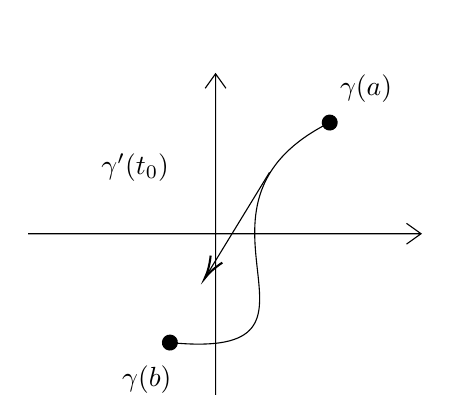
\begin{tikzpicture}[x=0.75pt,y=0.75pt,yscale=-1,xscale=1]
        %uncomment if require: \path (0,286); %set diagram left start at 0, and has height of 286
        
        %Shape: Axis 2D [id:dp5992461788507699] 
        \draw  (50,141.08) -- (239.26,141.08)(140.26,64) -- (140.26,226.51) (232.26,136.08) -- (239.26,141.08) -- (232.26,146.08) (135.26,71) -- (140.26,64) -- (145.26,71)  ;
        %Curve Lines [id:da8169369769076535] 
        \draw    (118.26,193.51) .. controls (210.26,202.51) and (113.26,128.51) .. (195.26,87.51) ;
        \draw [shift={(195.26,87.51)}, rotate = 333.43] [color={rgb, 255:red, 0; green, 0; blue, 0 }  ][fill={rgb, 255:red, 0; green, 0; blue, 0 }  ][line width=0.75]      (0, 0) circle [x radius= 3.35, y radius= 3.35]   ;
        \draw [shift={(118.26,193.51)}, rotate = 5.59] [color={rgb, 255:red, 0; green, 0; blue, 0 }  ][fill={rgb, 255:red, 0; green, 0; blue, 0 }  ][line width=0.75]      (0, 0) circle [x radius= 3.35, y radius= 3.35]   ;
        %Straight Lines [id:da7279313778056917] 
        \draw    (166.26,111.51) -- (136.05,160.92) ;
        \draw [shift={(135,162.63)}, rotate = 301.44] [color={rgb, 255:red, 0; green, 0; blue, 0 }  ][line width=0.75]    (10.93,-3.29) .. controls (6.95,-1.4) and (3.31,-0.3) .. (0,0) .. controls (3.31,0.3) and (6.95,1.4) .. (10.93,3.29)   ;
        
        % Text Node
        \draw (199,63.4) node [anchor=north west][inner sep=0.75pt]    {$\gamma ( a)$};
        % Text Node
        \draw (94,203.4) node [anchor=north west][inner sep=0.75pt]    {$\gamma ( b)$};
        % Text Node
        \draw (84,101.4) node [anchor=north west][inner sep=0.75pt]    {$\gamma '( t_{0})$};
        
        
        \end{tikzpicture}
\]

\defn Parameterize $\gamma(t)=(x(t), y(t))=x(t)+iy(t)$. Then $\gamma'(t_0)=(x'(t_0), y'(t_0))$ is a \textbf{tangent vector} to the curve at $\gamma(t_0)$ (assume $\gamma'(t_0)\neq \mathbf{0}$, aka. $\gamma$ is regular at $\gamma(t_0)$.)

\begin{theorem}[The ``Boxy-path'' Theorem]
    A nonempty open set $\Omega$ in $\C$ is connected \textit{if and only if} each pair of distinct
points in $\Omega$ can be joined by a sequence of line segments lying in $\Omega$, each of which is
parallel to either to the real or imaginary axis.
    \drawing{0.6\linewidth}{image-3.png}
    In other words, between any 2 points in a region $\reg$ there exists a ``\textbf{boxy path}''.
\end{theorem}

\rmk There is also always a \textbf{smooth path}. That is: \drawing{150pt}{image-4.png}

\begin{theorem}[``Smooth-path'']
    A nonempty open set $\reg$ in $\C$ is connected if and only if each pair of distinct
points in $\reg$ can be joined by a continuously differentiable curve in $\reg$ that is regular at
every point.
\end{theorem}
\begin{proof}
    See \href{https://stephangarcia.sites.pomona.edu/teaching/24S-135/Lecture/24S-135-Lecture02.pdf}{lecture 2 notes}.
\end{proof}

\subsection{Conformality}
Let $f$ be an analytic complex function on $\reg$.

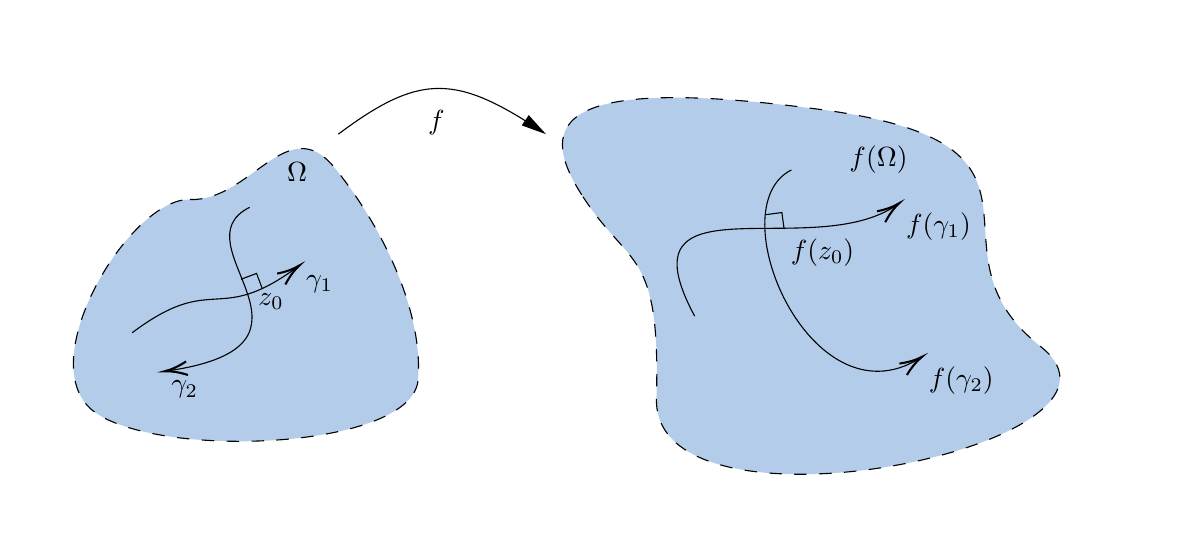
\begin{tikzpicture}[x=0.75pt,y=0.75pt,yscale=-1,xscale=1]
    %uncomment if require: \path (0,300); %set diagram left start at 0, and has height of 300
    
    %Shape: Polygon Curved [id:ds04152892949921583] 
    \draw  [fill={rgb, 255:red, 0; green, 87; blue, 184 }  ,fill opacity=0.3 ][dash pattern={on 4.5pt off 4.5pt}] (92.5,102.5) .. controls (121.5,103.5) and (139.5,59.5) .. (162,87) .. controls (184.5,114.5) and (204.91,155.75) .. (202.42,189.25) .. controls (199.92,222.75) and (79.59,227.75) .. (47.08,205.25) .. controls (14.58,182.75) and (63.5,101.5) .. (92.5,102.5) -- cycle ;
    %Curve Lines [id:da38490573070321243] 
    \draw    (64.67,166.67) .. controls (104.27,136.97) and (105.24,163.7) .. (144.07,135.13) ;
    \draw [shift={(145.25,134.25)}, rotate = 143.13] [color={rgb, 255:red, 0; green, 0; blue, 0 }  ][line width=0.75]    (10.93,-3.29) .. controls (6.95,-1.4) and (3.31,-0.3) .. (0,0) .. controls (3.31,0.3) and (6.95,1.4) .. (10.93,3.29)   ;
    %Curve Lines [id:da9683797356751562] 
    \draw    (121.25,106.25) .. controls (85.43,124.16) and (167.43,172.76) .. (81.56,185.07) ;
    \draw [shift={(80.25,185.25)}, rotate = 352.23] [color={rgb, 255:red, 0; green, 0; blue, 0 }  ][line width=0.75]    (10.93,-3.29) .. controls (6.95,-1.4) and (3.31,-0.3) .. (0,0) .. controls (3.31,0.3) and (6.95,1.4) .. (10.93,3.29)   ;
    %Shape: Right Angle [id:dp0014762610750393979] 
    \draw   (117.1,140.91) -- (124.59,138.1) -- (127.4,145.59) ;
    %Shape: Polygon Curved [id:ds020760136591730705] 
    \draw  [fill={rgb, 255:red, 0; green, 87; blue, 184 }  ,fill opacity=0.3 ][dash pattern={on 4.5pt off 4.5pt}] (281.25,100.25) .. controls (258.25,64.25) and (271.25,42.25) .. (397.25,59.25) .. controls (523.25,76.25) and (442.25,126.25) .. (502.25,173.25) .. controls (562.25,220.25) and (315.25,271.25) .. (317.25,198.25) .. controls (319.25,125.25) and (304.25,136.25) .. (281.25,100.25) -- cycle ;
    %Curve Lines [id:da5067199553805877] 
    \draw    (335.67,158.67) .. controls (298.63,89.94) and (392.35,133.36) .. (433.04,105.13) ;
    \draw [shift={(434.25,104.25)}, rotate = 143.13] [color={rgb, 255:red, 0; green, 0; blue, 0 }  ][line width=0.75]    (10.93,-3.29) .. controls (6.95,-1.4) and (3.31,-0.3) .. (0,0) .. controls (3.31,0.3) and (6.95,1.4) .. (10.93,3.29)   ;
    %Curve Lines [id:da12902529814050778] 
    \draw    (382.25,88.25) .. controls (346.61,106.07) and (391.34,211.12) .. (443.67,179.26) ;
    \draw [shift={(445.25,178.25)}, rotate = 146.56] [color={rgb, 255:red, 0; green, 0; blue, 0 }  ][line width=0.75]    (10.93,-3.29) .. controls (6.95,-1.4) and (3.31,-0.3) .. (0,0) .. controls (3.31,0.3) and (6.95,1.4) .. (10.93,3.29)   ;
    %Shape: Right Angle [id:dp16473621622546486] 
    \draw   (369.76,109.81) -- (377.69,108.76) -- (378.75,116.69) ;
    %Curve Lines [id:da7241992906101147] 
    \draw    (164,71) .. controls (203.6,41.3) and (220.91,42.23) .. (262.73,70.15) ;
    \draw [shift={(264,71)}, rotate = 213.92] [fill={rgb, 255:red, 0; green, 0; blue, 0 }  ][line width=0.08]  [draw opacity=0] (12,-3) -- (0,0) -- (12,3) -- cycle    ;
    
    % Text Node
    \draw (138,83.4) node [anchor=north west][inner sep=0.75pt]    {$\Omega $};
    % Text Node
    \draw (147.25,137.65) node [anchor=north west][inner sep=0.75pt]    {$\gamma _{1}$};
    % Text Node
    \draw (82.25,188.65) node [anchor=north west][inner sep=0.75pt]    {$\gamma _{2}$};
    % Text Node
    \draw (124.25,146.65) node [anchor=north west][inner sep=0.75pt]    {$z_{0}$};
    % Text Node
    \draw (409,75.4) node [anchor=north west][inner sep=0.75pt]    {$f( \Omega )$};
    % Text Node
    \draw (436.25,107.65) node [anchor=north west][inner sep=0.75pt]    {$f( \gamma _{1})$};
    % Text Node
    \draw (447.25,181.65) node [anchor=north west][inner sep=0.75pt]    {$f( \gamma _{2})$};
    % Text Node
    \draw (380.75,120.09) node [anchor=north west][inner sep=0.75pt]    {$f( z_{0})$};
    % Text Node
    \draw (206,58.4) node [anchor=north west][inner sep=0.75pt]    {$f$};
    
    
\end{tikzpicture}

Let $z_0\in \reg$ such that $f'(z_0)\neq 0$. Let $\gamma_1, \gamma_2$ be two curves that pass through $z_0$ intersecting with an angle $\theta$. Then $f(\gamma_1), f(\gamma_2)$ are two curves in $f(\Omega)$ passing through $f(\zeta_0)$ also with angle $\theta$.

Therefore, $f$ is \textbf{conformal}!

\section{Cauchy-Riemann equations, harmonic functions}
\subsection{Multivariate notion of complex derivatives}
Recall: $\displaystyle f'(z_0)=\lim_{h\to 0}\frac{f(z_0+h)-f(z_0)}{h}$.

Now we write each function with complex variables as $f(z)=u(z)+i\, v(z)$ where $u,v$ are real-valued \sidenote{meaning their range is real} functions.

Since $\C\cong \R^2$, we denote every point $z=(x,y)$.

Now we let $f(x,y)=u(x,y)+i\,v(x,y)$. We first let the small distance $h=(r,0)$ be horizontally approaching 0 with $r\in \R$. That is, $z_0+h=(x_0+r,y_0)$.
\begin{align*}
    f'(z_0) &= \lim_{r\to 0} \frac{u(x_0+r, y_0)-u(x_0,y_0)}{r} + i\cdot \lim_{r\to 0}\frac{v(x_0+r, y_0)-v(x_0,y_0)}{r}\\
    &=u_x(x_0,y_0)+i\cdot v_x(x_0,y_0)
\end{align*}

Similarly, if we vertically let $h=ir=(0,r)$ with $r\to 0, r\in \R$, we would get $f'=v_y-i\cdot u_y$.

\rmk If a derivative exists, the horizontal \& the vertical ones should be equal!

\begin{theorem}[Cauchy-Riemann Equations]
    \begin{align*}
        u_x &=v_y\\
        u_y &= -v_x
    \end{align*}
\end{theorem}\addlink{Cauchy-Riemann Equations}

\begin{corollary}
    If $f:\reg \to \C$ is analytic and $f'=0$ on $\reg$, then $f$ is \textbf{constant}.
\end{corollary}
\begin{proof}
    Since $0=f'=u_x+iv_x$, we see that $u_x=v_x=0$ on $\reg$. By Cauchy-Riemann, $v_y=u_y=0$ is also true on $\reg$. Hence, $\mathbf{u}, \mathbf{v}$ are constant on either horizontal or vertical segments. By the Boxy Path Theorem, $f=u+iv$ cannot assume two distinct values in $\reg$.
\end{proof}

\subsection{Orientation-preserving as shown by Jacobian}
Let $f:\reg \to \C$ be analytic. Then $f'=u_x+iv_x$ and hence:\begin{align*}
    |f'|^2 = \bar f'\cdot f &= (u_x-iv_x)(u_x+iv_x)\\
    &= u_x^2 + v_x^2\\
    &= u_xu_x+v_xv_x && \text{and by Cauchy-Riemann,}\\
    &= u_xv_y-u_yv_x\\
    &= \det\left(\begin{bmatrix}
        u_x & u_y\\
        v_x & v_y
    \end{bmatrix}\right) && \text{the Jacobian of $f$!}
\end{align*}

Since $|f'|^2\geq 0$, the determinant of the Jacobian is always $\geq 0$, implying that $f$ is always locally orientation-preserving. Moreover,

\begin{proposition}
    If $f'(z_0)\neq 0$, then $|f'|^2> 0$ implies:
    \begin{enumerate}
        \item $f$ is \textbf{injective} near $z_0$
        \item $f$ scales $\R$ by $|f'(z_0)|^2$ near $z_0$
        \item $f$ preserves orientation near $z_0$
    \end{enumerate}
\end{proposition}

\subsection{The Laplacian, harmonic functions and conjugates}
Suppose that $f=u+iv$ is analytic and $u,v$ have continuous second partial derivatives. Then:\begin{align*}
    u_{xx}+u_{yy} = \Delta u = (v_y)_x + (-v_x)_y = v_{yx}-v_{xy}=0
\end{align*}
This means that the Laplacian of this function $u$ is 0!\sidenote{$\Delta u = 0$ characterizes steady-state solutions to heat equations on $\reg$.}

\defn Real-valued functions $u: \reg\to \R$ satisfying that the Laplacian $\Delta u= u_{xx}+u_{yy}$ is 0 on $\reg$ is called \textbf{harmonic functions}.

\defn A \textbf{harmonic conjugate} of $u$ is a harmonic function $v: \reg \to \R$ such that $f=u+i\cdot v$ is \textbf{analytic} on $\reg$.
\addlink{Harmonic conjugate}

\eg $u=x^2-y^2, v=2xy$.\sidenote{Check it!}

\rmk Harmonic conjugates are unique up to translation (± constants).

\rmk If $u$ is harmonic on $\reg$, it does NOT have to have a harmonic conjugate on $\reg$.

\subsection{Finding a harmonic conjugate}
Recall that the real and imaginary parts of an analytic function are \textbf{harmonic}, in addition to satisfying the Cauchy-Riemann Equations: $u_x=v_y$ and $u_y=-v_x$.

\eg $u(z)=\log |z|$ is harmonic on $\C\backslash\{0\}$.
\begin{proof}
    Write $u(x,y)=\log (\sqrt{x^2+y^2})=\frac{1}{2}\log(x^2+y^2)$.

    Then, \begin{align*}
        u_x&=\frac{\partial}{\partial x}\left(\frac{1}{2}\log (x^2+y^2)\right)\\
        &= \frac{1}{2}\cdot \frac{2x}{x^2+y^2}\\
        &= \frac{x}{x^2+y^2}
    \end{align*}

    Hence,\sidenote{Review quotient rule!}
    \begin{align*}
        u_{xx} &= \frac{(x^2+y^2)-x(2x)}{(x^2+y^2)^2}\\
        &= \frac{y^2-x^2}{(x^2+y^2)^2}
    \end{align*}

    Symmetrically, we find \begin{align*}
        u_{yy} & = \frac{x^2-y^2}{(x^2+y^2)^2}
    \end{align*}
    Hence $u_{xx}+u_{yy}=0$, implying that the function is harmonic.
\end{proof}

Now, can we \uline{find a harmonic conjugate for the aforementioned $u$}?\sidenote{There is currently a great \textbf{CAVEAT} in all of these, because $v(z)=\arg(z)$ cannot be defined in a continuous manner in all of $\C\backslash\{0\}$: 

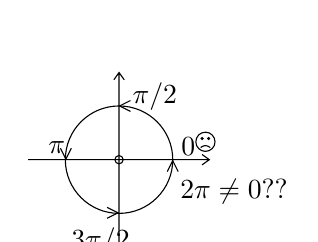
\begin{tikzpicture}[x=0.75pt,y=0.75pt,yscale=-0.5,xscale=0.5]
    %uncomment if require: \path (0,300); %set diagram left start at 0, and has height of 300
    
    %Shape: Axis 2D [id:dp48156480156165227] 
    \draw  (111,139) -- (285.5,139)(198.5,55) -- (198.5,219) (278.5,134) -- (285.5,139) -- (278.5,144) (193.5,62) -- (198.5,55) -- (203.5,62)  ;
    %Shape: Circle [id:dp6012967995903811] 
    \draw   (146.75,139) .. controls (146.75,110.42) and (169.92,87.25) .. (198.5,87.25) .. controls (227.09,87.25) and (250.26,110.42) .. (250.26,139) .. controls (250.26,167.58) and (227.09,190.75) .. (198.5,190.75) .. controls (169.92,190.75) and (146.75,167.58) .. (146.75,139) -- cycle ;
    \draw   (209.5,92.5) -- (199,87.25) -- (209.5,82) ;
    \draw   (152.5,128) -- (147.25,138.5) -- (142,128) ;
    \draw   (187,185) -- (197.5,190.25) -- (187,195.5) ;
    \draw   (245,150.5) -- (250.25,140) -- (255.5,150.5) ;
    %Shape: Smiley Face [id:dp013237994815757492] 
    \draw   (272.5,121.75) .. controls (272.5,116.64) and (276.64,112.5) .. (281.75,112.5) .. controls (286.86,112.5) and (291,116.64) .. (291,121.75) .. controls (291,126.86) and (286.86,131) .. (281.75,131) .. controls (276.64,131) and (272.5,126.86) .. (272.5,121.75) -- cycle ; \draw   (277.68,118.61) .. controls (277.68,118.09) and (278.09,117.68) .. (278.61,117.68) .. controls (279.12,117.68) and (279.53,118.09) .. (279.53,118.61) .. controls (279.53,119.12) and (279.12,119.53) .. (278.61,119.53) .. controls (278.09,119.53) and (277.68,119.12) .. (277.68,118.61) -- cycle ; \draw   (283.97,118.61) .. controls (283.97,118.09) and (284.38,117.68) .. (284.9,117.68) .. controls (285.41,117.68) and (285.82,118.09) .. (285.82,118.61) .. controls (285.82,119.12) and (285.41,119.53) .. (284.9,119.53) .. controls (284.38,119.53) and (283.97,119.12) .. (283.97,118.61) -- cycle ; \draw   (277.13,127.3) .. controls (280.21,124.83) and (283.29,124.83) .. (286.38,127.3) ;
    %Shape: Circle [id:dp5943162664556252] 
    \draw   (194.51,139) .. controls (194.51,136.79) and (196.3,135) .. (198.5,135) .. controls (200.71,135) and (202.5,136.79) .. (202.5,139) .. controls (202.5,141.21) and (200.71,143) .. (198.5,143) .. controls (196.3,143) and (194.51,141.21) .. (194.51,139) -- cycle ;
    
    % Text Node
    \draw (256,115.4) node [anchor=north west][inner sep=0.75pt]    {$0$};
    % Text Node
    \draw (209,62.4) node [anchor=north west][inner sep=0.75pt]    {$\pi /2$};
    % Text Node
    \draw (128,119.4) node [anchor=north west][inner sep=0.75pt]    {$\pi $};
    % Text Node
    \draw (150,202.4) node [anchor=north west][inner sep=0.75pt]    {$3\pi /2$};
    % Text Node
    \draw (255,155.4) node [anchor=north west][inner sep=0.75pt]    {$2\pi \neq 0??$};
    
    
    \end{tikzpicture}
    

To be resolved later!}

We could use the two Cauchy-Riemann Equations. One of them:
\begin{align*}
    v_y&=u_x\\
    &= \frac{x}{x^2+y^2}
\end{align*}
Therefore, \begin{align*}
    v(x,y) &= \int v_ydy + C(x) && \text{unknown function of }x\\
    &= \arctan\left(\frac{y}{x}\right)+C(x)
\end{align*}

Then, we use the second one: \begin{align*}
    \frac{y}{x^2+y^2}=u_y=-v_x &= -\frac{\partial}{\partial x} \left( \arctan\left(\frac{y}{x}\right)+C(x)\right)\\
    &= \frac{y}{x^2+y^2}-C'(x) \implies C'(x)=0
\end{align*}

Hence, a good harmonic conjugate candidate seems to be \begin{align*}
    v(x,y) = \arctan\left(\frac{y}{x}\right) + C
\end{align*}
where $C$ is a constant. WLOG, let $C=0$. Then $ v(x,y)=\arctan\left(\frac{y}{x}\right)$, meaning that: \begin{align*}
    v(z)=\arg (z)
\end{align*}

Therefore, $f(z)=\log |z| + i\cdot \arg(z)$ is analytic!
%%%%%%%

\subsection{Physics analogies of harmonic functions}
\eg Let $T(x,y,t)$ be the temperature at $(x,y)$ at time $t$ of a thermally conductive plate in $\C$. Assume the plate gives rise to a \textbf{bounded} region $\Omega$ (with boundary denoted $\partial \Omega$). Temperature on $\partial \Omega$ is a fixed function (time-independent).

\begin{figure}[H]
    \centering
    
\includegraphics[width=80pt]{Images/image-2.png}
\end{figure}

Now given the heat equation: \begin{align*}
    \frac{\partial T}{\partial t}-\alpha \Delta T=0
\end{align*}
where $\alpha$ is a constant.

We think the system tends towards a thermal equilibrium as $t\to \infty$. At equilibrium, $\frac{\partial T}{\partial t}$ is \textbf{zero}. Hence, at equilibrium, $\Delta T=T_{xx}+T_{yy}=0$.

\textbf{\underline{Idea}}: Harmonic function behave like equilibrium temperature distributions!

\begin{proposition}
    Let $U(x,y)$ be a harmonic function on $\Omega$.
    \begin{enumerate}
        \item $U$ cannot have a \textit{local} maximum in $\Omega$.
        \item The absolute maximum of $U$ on $\Omega ^-$\sidenote{$\Omega ^-$ denotes the closure of $\Omega$} occurs on $\partial \Omega$.
        \item $U$ cannot be locally constant without being globally constant.
    \end{enumerate}
\end{proposition}

\begin{theorem}[Maximum principle]
    Let $\Omega$ be a bounded region in $\C$ and let $f: \Omega^-\to \C$ be analytic on $\Omega$ and continuous on $\Omega^-$.
    \begin{enumerate}
        \item If $|f|$ achieves a local max in $\Omega$, then $f$ is constant.
        \item The global max of $|f|$ on $\Omega^-$ is attained on $\partial \Omega$.
    \end{enumerate}
\end{theorem}

\section{Möbius transformations}
\subsection{Möbius transformations, the extended plane}
\defn[Möbius transformations]
\begin{align*}
    f(z)=\frac{az+b}{cz+d}\text{ where } ad-bc\neq 0, a,b,c,d\in \C
\end{align*}
Such an $f$ is \textbf{analytic} on $\C\backslash\{\frac{-d}{c}\}$\sidenote{recall that rational functions are analytic except when the denominator vanishes, i.e. $cz+d\neq 0$.} and \textbf{comformal} there since $f'(z)=\frac{ad-bc}{(cz+d)^2}\neq 0$ on $\C\backslash\{\frac{-d}{c}\}$.

\rmk In addition, $f$ is injective (one-to-one)!
\begin{proof}
    \begin{align*}
        f(z)=f(w)\implies \frac{az+b}{cz+d}&=\frac{aw+b}{cw+d}\\
         (az+b)(cw+d)&= (cz+d)(aw+b)\\
         aczw+bcw+adz+bd&=aczw+adw+bcz+bd\\
         (ad-bc)z&=(ad-bc)w\\
         z&=w
    \end{align*}
\end{proof}

\defn[The extended plane] We set the following convention:\begin{align*}
    f(\frac{-d}{c})&= \infty\\
    f(\infty) &= \frac{a}{c}
\end{align*}
with this, $f$ is a \textbf{bijection} from $\Chat=\C\cup\{\infty\}$ to itself.\sidenote{recall Riemann sphere}

\subsection{Möbius transformations as matrices}
\rmk We can \textit{associate}\sidenote{this association is not a bijection: it's only so up to scaling} $f(z)=\frac{az+b}{cz+d}$ where $ad-bc\neq 0$ with the matrix $$M_f=\begin{bmatrix}
    a&b\\c&d
\end{bmatrix}$$

\rmk $M_{f\circ g}=M_f\cdot M_g$\sidenote{check this!}

\rmk The inverse of $M_f=\begin{bmatrix}
    a&b\\c&d
\end{bmatrix}$ is $M_f^{-1}=\frac{1}{ad-bc}\begin{bmatrix}
    d&-b\\-c&a
\end{bmatrix}$ and scaling does not matter, so we could write the \textbf{inverse} of such Möbius transformation as: \begin{align*}
    \inv{f}(w) &=\frac{dw-b}{-cw+a}
\end{align*}

\begin{theorem}
    A Möbius transformation $f:\Chat\to\Chat$ with three fixed points in $\Chat$ is the \textbf{identity map} $\mathrm{id}(z)=z=\frac{z+0}{0z+1}$.\sidenote{$I=\begin{bmatrix}
        1&0\\0&1
    \end{bmatrix}$}
\end{theorem}
\begin{proof}
    Let $f(z)=\frac{az+b}{cz+d}$ be a Möbius transformation.
    \begin{enumerate}
        \item If $\infty$ is fixed, then $c=0$\sidenote{think about that!}. Then $f(z)=\frac{a}{d}z+\frac{b}{d}$, which is a \textbf{linear} transformation.\begin{enumerate}
            \item If $f(z)=z$, we are done since we get the identity!
            \item Otherwise the function only has one fixed point at $\infty$.
        \end{enumerate}
        \item If $\infty$ is not a fixed point, then $c\neq 0$. Solve:\begin{align*}
            f(z)+z \Leftrightarrow \frac{az+b}{cz+d}&=z\\
            az+b&=cz^2+dz\\
            cz^2+(d-a)z-b&=0
        \end{align*}
        is a quadratic which has at most two (distinct) solutions in $\C$. Hence, this transformation fixes at most two points.
    \end{enumerate}
\end{proof}

\subsection{Möbius transformations take circles to circles}
\rmk Lines can be circles (they are just circles that pass through the point at infinity).

\begin{theorem}
    The image of a circle under a Möbius transformation is still a circle.
\end{theorem}
\begin{proof}
    Let $f(z)=\frac{az+b}{cz+d}$ be a Möbius transformation.
    \begin{enumerate}
        \item If $c=0$, then $f(z)=\frac{a}{d}z+\frac{b}{d}$, which is a \textbf{linear/affine} transformation and so we are done\sidenote{since linear transformations preserve circles and lines}.
        \item Now suppose $c\neq 0$. Then \begin{align*}
            f(z)&=\frac{a}{d}z+\frac{b}{d}\\
            &= \frac{\frac{a}{c}(cz+d)-\frac{ad}{c}+b}{cz+d}\\
            &= \frac{b-\frac{ad}{c}}{cz+d}+\frac{a}{c}
        \end{align*}
        which is a composition of affine, inversion and affine:
        $$z\mapsto cz+d\mapsto \frac{1}{cz+d}\mapsto \frac{b-\frac{ad}{c}}{cz+d}+\frac{a}{c}$$
        We now only need to show that inversion preserves circles.

        Let a circle in $\R^2$ be $Ax+By+C(x^2+y^2)=D$ where $A,B,C,D\in \R$. If $z=x+iy\in \Chat$, then $\frac{1}{z}=\frac{x}{x^2+y^2}+i\frac{-y}{x^2+y^2}$. Name $\frac{1}{z}=u+iv$, note that $u^2+v^2=\frac{1}{x^2+y^2}$. 
        
        Then we note that $Au-Bv+C=D(u^2+v^2)$\sidenote{check this!}, which is still a circle!
    \end{enumerate}
\end{proof}

\begin{theorem}
    Given two triples $z_1,z_2,z_3$ and $w_1,w_2,w_3$ of \textit{distinct} points in $\Chat$, then there is always a unique Möbius transformation $f$ such that $f(z_i)=w_i$ for all $i=1,2,3$.
\end{theorem}
\begin{proof}
    Claim: the \textit{cross-ratio} $\phi(z)=\frac{z-z_1}{z-z_3}\cdot \underset{\text{const.}}{\underbrace{\frac{z_2-z_3}{z_2-z_1}}}$ is a Möbius transformation that satisfies \circled{$\phi(z_1)=0, \phi(z_2)=1, \phi(z_3)=\infty$}.

    We can also find another Möbius transformation such that $\psi(z_1)=0, \psi(z_2)=1, \psi(z_3)=\infty$. Then:
    \[\begin{tikzcd}[ampersand replacement=\&,cramped,row sep=tiny]
        {z_1} \& 0 \& {w_1} \\
        {z_2} \& 1 \& {w_2} \\
        {z_3} \& \infty \& {w_3}
        \arrow["\phi", maps to, from=1-1, to=1-2]
        \arrow["{\psi^{-1}}", maps to, from=1-2, to=1-3]
        \arrow["\phi", maps to, from=2-1, to=2-2]
        \arrow["{\psi^{-1}}", maps to, from=2-2, to=2-3]
        \arrow["\phi", maps to, from=3-1, to=3-2]
        \arrow["{\psi^{-1}}", maps to, from=3-2, to=3-3]
    \end{tikzcd}\]

    and we could simply let $f=\psi^{-1}\circ \phi$.
\end{proof}

\eg Let $f(z)=\frac{z+1}{-z+1}$. We compute:\begin{align*}
    f(0)&=1\\
    f(-1)&=0\\
    f(1)&=\infty\\
    f(i)&=i\\
    f(-i)&=-i\\
\end{align*}

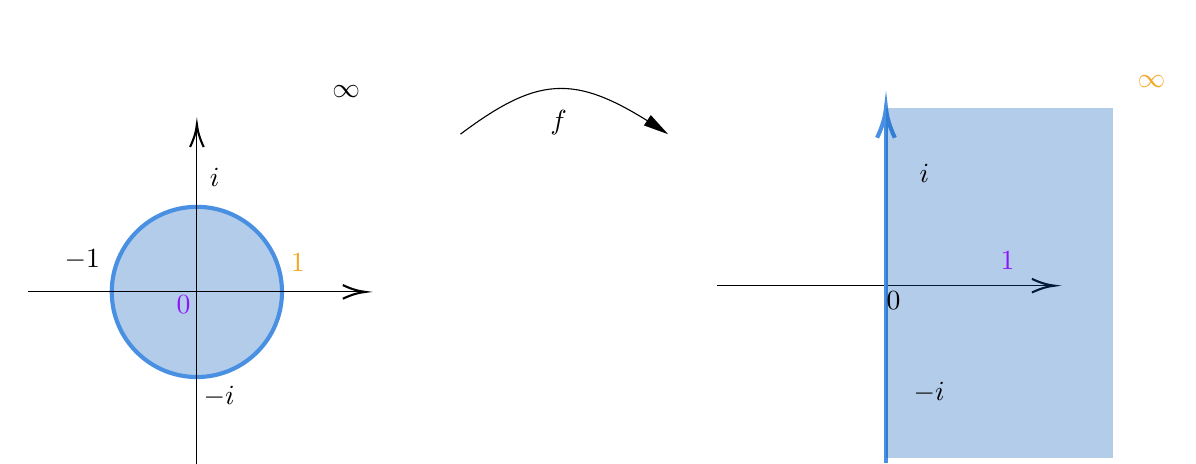
\begin{tikzpicture}[x=0.75pt,y=0.75pt,yscale=-1,xscale=1]
%uncomment if require: \path (0,300); %set diagram left start at 0, and has height of 300

%Shape: Circle [id:dp46487660565461075] 
\draw  [color={rgb, 255:red, 74; green, 144; blue, 226 }  ,draw opacity=1 ][fill={rgb, 255:red, 0; green, 87; blue, 184 }  ,fill opacity=0.3 ][line width=1.5]  (96,156.01) .. controls (96,133.37) and (114.36,115.01) .. (137.01,115.01) .. controls (159.65,115.01) and (178.01,133.37) .. (178.01,156.01) .. controls (178.01,178.66) and (159.65,197.02) .. (137.01,197.02) .. controls (114.36,197.02) and (96,178.66) .. (96,156.01) -- cycle ;
%Curve Lines [id:da6037660096213038] 
\draw    (264,80) .. controls (303.6,50.3) and (320.91,51.23) .. (362.73,79.15) ;
\draw [shift={(364,80)}, rotate = 213.92] [fill={rgb, 255:red, 0; green, 0; blue, 0 }  ][line width=0.08]  [draw opacity=0] (12,-3) -- (0,0) -- (12,3) -- cycle    ;
%Straight Lines [id:da30485423184171] 
\draw    (55.75,156.01) -- (216.26,156.01) ;
\draw [shift={(218.26,156.01)}, rotate = 180] [color={rgb, 255:red, 0; green, 0; blue, 0 }  ][line width=0.75]    (10.93,-3.29) .. controls (6.95,-1.4) and (3.31,-0.3) .. (0,0) .. controls (3.31,0.3) and (6.95,1.4) .. (10.93,3.29)   ;
%Straight Lines [id:da03496103337291223] 
\draw    (387.75,153.01) -- (548.26,153.01) ;
\draw [shift={(550.26,153.01)}, rotate = 180] [color={rgb, 255:red, 0; green, 0; blue, 0 }  ][line width=0.75]    (10.93,-3.29) .. controls (6.95,-1.4) and (3.31,-0.3) .. (0,0) .. controls (3.31,0.3) and (6.95,1.4) .. (10.93,3.29)   ;
%Straight Lines [id:da11880027193931353] 
\draw    (137.01,246.26) -- (137.01,77.26) ;
\draw [shift={(137.01,75.26)}, rotate = 90] [color={rgb, 255:red, 0; green, 0; blue, 0 }  ][line width=0.75]    (10.93,-3.29) .. controls (6.95,-1.4) and (3.31,-0.3) .. (0,0) .. controls (3.31,0.3) and (6.95,1.4) .. (10.93,3.29)   ;
%Straight Lines [id:da4256972022746721] 
\draw [color={rgb, 255:red, 74; green, 144; blue, 226 }  ,draw opacity=1 ][line width=1.5]    (469.01,238.51) -- (469.01,70.51) ;
\draw [shift={(469.01,67.51)}, rotate = 90] [color={rgb, 255:red, 74; green, 144; blue, 226 }  ,draw opacity=1 ][line width=1.5]    (14.21,-4.28) .. controls (9.04,-1.82) and (4.3,-0.39) .. (0,0) .. controls (4.3,0.39) and (9.04,1.82) .. (14.21,4.28)   ;
%Shape: Rectangle [id:dp17327106892852906] 
\draw  [draw opacity=0][fill={rgb, 255:red, 0; green, 87; blue, 184 }  ,fill opacity=0.3 ] (469.01,67.51) -- (578.26,67.51) -- (578.26,236.26) -- (469.01,236.26) -- cycle ;

% Text Node
\draw (142,95.4) node [anchor=north west][inner sep=0.75pt]    {$i$};
% Text Node
\draw (181,136.4) node [anchor=north west][inner sep=0.75pt]  [color={rgb, 255:red, 245; green, 166; blue, 35 }  ,opacity=1 ]  {$1$};
% Text Node
\draw (139.01,200.42) node [anchor=north west][inner sep=0.75pt]    {$-i$};
% Text Node
\draw (72,134.4) node [anchor=north west][inner sep=0.75pt]    {$-1$};
% Text Node
\draw (126,156.4) node [anchor=north west][inner sep=0.75pt]  [color={rgb, 255:red, 144; green, 19; blue, 254 }  ,opacity=1 ]  {$0$};
% Text Node
\draw (484,93.4) node [anchor=north west][inner sep=0.75pt]    {$i$};
% Text Node
\draw (523,135.4) node [anchor=north west][inner sep=0.75pt]  [color={rgb, 255:red, 144; green, 19; blue, 254 }  ,opacity=1 ]  {$1$};
% Text Node
\draw (481.01,198.42) node [anchor=north west][inner sep=0.75pt]    {$-i$};
% Text Node
\draw (468,154.4) node [anchor=north west][inner sep=0.75pt]    {$0$};
% Text Node
\draw (201,55.4) node [anchor=north west][inner sep=0.75pt]    {$\infty $};
% Text Node
\draw (306,67.4) node [anchor=north west][inner sep=0.75pt]    {$f$};
% Text Node
\draw (589,50.4) node [anchor=north west][inner sep=0.75pt]    {$\textcolor[rgb]{0.96,0.65,0.14}{\infty }$};


\end{tikzpicture}

\end{document} 
